
% Font and layout
\usepackage{times}
\usepackage[margin=1in]{geometry}
\usepackage{titlesec}
\titleformat{\section}[block]{\huge\bfseries\centering\underline}{}{0em}{}
\setcounter{secnumdepth}{0}
\usepackage{color}
\usepackage{amsmath}
\usepackage{listings}
\renewcommand{\ttdefault}{lmtt}
\usepackage{xstring}

% Graphics and floats
\usepackage{graphicx}
\usepackage{float}
\usepackage{tikz}
\usepackage{grfext}
\usetikzlibrary{calc}
\usepackage{subcaption}


% Tables
\usepackage{booktabs}
\usepackage{array}
\usepackage{multirow}
\usepackage{longtable}
\usepackage{tabularx}
\usepackage{makecell}
\usepackage{ragged2e}
\usepackage[table]{xcolor}

% Custom column types
\newcolumntype{M}[1]{>{\centering\arraybackslash}m{#1}}
\newcolumntype{L}[1]{>{\raggedright\arraybackslash}m{#1}}

% Landscape support
\usepackage{pdflscape}
\usepackage{lscape}

% Code and Sweave
\usepackage{Sweave}

% CSV tables
\usepackage{csvsimple}

% TOC formatting
\usepackage{tocloft}
\usepackage{titletoc}
\renewcommand{\cftsecleader}{\cftdotfill{\cftdotsep}}

% Hyperlinks
\usepackage{hyperref}

% Page style and headers/footers
\usepackage{fancyhdr}
\usepackage{lastpage}
\pagestyle{fancy}
\fancyhf{}
\rhead{\thepage}
\lhead{Your Document Title or Section}
\renewcommand{\headrulewidth}{0.4pt}

% Horizontal rule command
\newcommand\HRule{\rule{\textwidth}{1pt}}

% Table Commands
\newcommand{\justiceTable}[2]{ % #1 = CSV file path, #2 = Caption
\begin{table}[H]
    \centering
    \renewcommand{\arraystretch}{1.5} % Add space between data rows
    \caption{#2}
    \vspace{2mm}
    \csvreader[
        tabular= {>{\centering\arraybackslash}p{0.25\textwidth} *{9}{>{\centering\arraybackslash}c}},
        table head = {
            \toprule
            \multicolumn{1}{c}{} &
            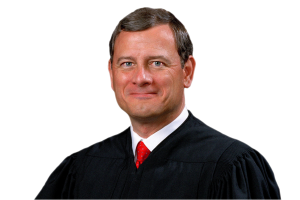
\includegraphics[width=1.75cm]{"images/justice_images/Roberts.png"} &
            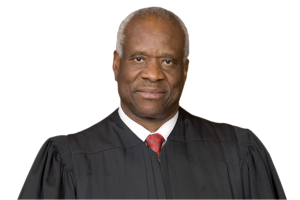
\includegraphics[width=1.75cm]{"images/justice_images/Thomas.png"} &
            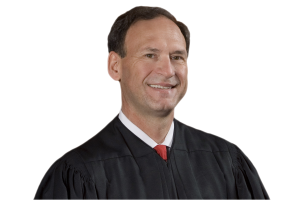
\includegraphics[width=1.75cm]{"images/justice_images/Alito.png"} &
            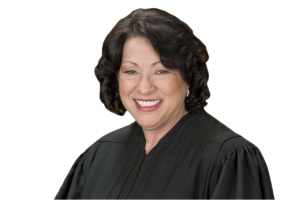
\includegraphics[width=1.75cm]{"images/justice_images/Sotomayor.png"} &
            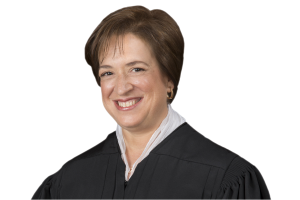
\includegraphics[width=1.75cm]{"images/justice_images/Kagan.png"} &
            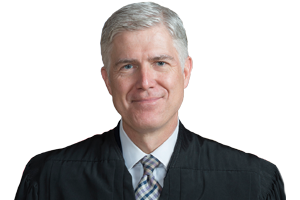
\includegraphics[width=1.75cm]{"images/justice_images/Gorsuch.png"} &
            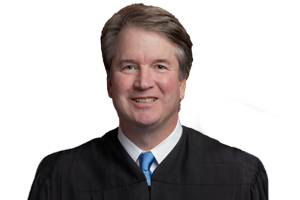
\includegraphics[width=1.75cm]{"images/justice_images/Kavanaugh.png"} &
            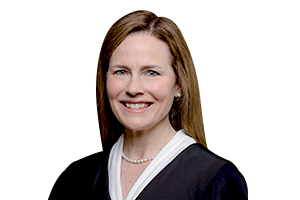
\includegraphics[width=1.75cm]{"images/justice_images/Barrett.png"} &
            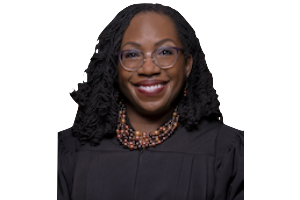
\includegraphics[width=1.75cm]{"images/justice_images/Jackson.png"} \rule[-2ex]{0pt}{0pt} \\[-2ex]
            \textbf{Case} & \textbf{Roberts} & \textbf{Thomas} & \textbf{Alito} & \textbf{Sotomayor} & \textbf{Kagan} & \textbf{Gorsuch} & \textbf{Kavanaugh} & \textbf{Barrett} & \textbf{Jackson} \\
            \cmidrule{1-10}
        },
        table foot = \bottomrule \\
    ]{#1}{}{
        \StrGobbleLeft{\csvcoli}{1}[\StrTemp]%
        \StrGobbleRight{\StrTemp}{1}[\CleanColi]%
        \normalsize \CleanColi & \csvcoliii & \csvcoliv & \csvcolv & \csvcolvi & \csvcolvii & \csvcolviii & \csvcolix & \csvcolx & \csvcolxi
    }
\end{table}
}







